
\begin{name}
	{\tenchude}
	{ĐỀ KSCL-THPT LÊ THÁNH TÔNG-HCM-L1}
	{LỚP TOÁN THẦY PHÁT}
	{\lq\lq  Live life to the fullest, and focus on the positive.\rq\rq}
\end{name}
 

\Opensolutionfile{ansbook}[ans/ansb\currfilebase]
\caulc
\Opensolutionfile{ans}[ans/ans\currfilebase-Phan-I]
 %%%==============Cau_EX1==============%%%
\begin{ex}%[1D2N2-2]
	Cấp số cộng $\left(u_{n}\right)$ có $u_{1}=-1$ và $u_{2}=3$. Số hạng $u_{5}$ của cấp số cộng bằng
	\choice
	{\True $15$}
	{$5$}
	{$9$}
	{$13$}
	\loigiai{
		Ta có công sai $d = u_{2} - u_{1} = 3 - \left(-1\right) = 4$.\\
		Số hạng $u_{5} = u_{1} + 4d = -1 + 4 \cdot 4 = 15$.
	}
\end{ex}

\begin{ex}%[1D6N4-2]
	Tập nghiệm của bất phương trình $\log_{3}\left(x+1\right) \le 2$ là
	\choice
	{$\left(1;9\right)$}
	{$\left(-\infty;9\right]$}
	{$\left(-1;7\right]$}
	{\True $\left(-1;8\right]$}
	\loigiai{
		Điều kiện $x+1 > 0 \Leftrightarrow x > -1$.\\
		Ta có $\log_{3}\left(x+1\right) \le 2 \Leftrightarrow x+1 \le 3^2 \Leftrightarrow x \le 8$.\\
		Kết hợp điều kiện, tập nghiệm là $S = \left(-1;8\right]$.
	}
\end{ex}

\begin{ex}%[2D1N1-2]
	\immini[thm]{Cho hàm số có đồ thị $y = f\left(x\right)$ như hình vẽ bên dưới. Hàm số đã cho nghịch biến trên khoảng nào sau đây?
		\choice
		{$\left(-1; 1\right)$}
		{$\left(-\infty; 1\right)$}
		{\True $\left(-\infty; -1\right)$}
		{$\left(-1; +\infty\right)$}
	}{
		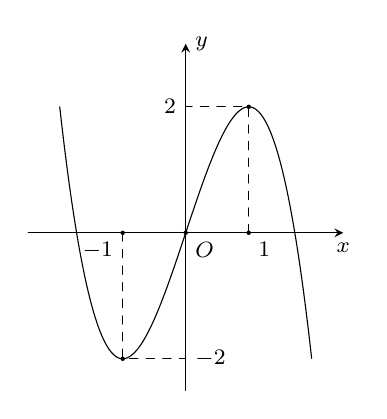
\begin{tikzpicture}[>=stealth,scale=0.8, font=\footnotesize, line join=round,line cap=round]
			% --- Thiết lập giới hạn khung hình ---
			\def\xmin{-2.5} \def\xmax{2.5}
			\def\ymin{-2.5} \def\ymax{3}
			
			% --- Hệ trục tọa độ ---
			\draw[->] (\xmin,0)--(\xmax,0) node[below]{$x$};
			\draw[->] (0,\ymin)--(0,\ymax) node[right]{$y$};
			\fill (0,0) circle (1pt) node[below right] {$O$};
			
			% --- Vẽ đồ thị hàm số y = -x^3 + 3x ---
			\begin{scope}
				\clip (\xmin,\ymin) rectangle (\xmax,\ymax);
				\draw[smooth, samples=150, domain=-2:2] plot (\x,{-(\x)^3 + 3*(\x)});
			\end{scope}
			
			% --- Các điểm đặc biệt ---
			% Điểm cực tiểu (-1, -2)
			\draw[dashed] (-1,0) node[below left]{$-1$} -- (-1,-2) -- (0,-2) node[right]{$-2$};
			\fill (-1,-2) circle (1pt);
			\fill (-1,0) circle (1pt);
			
			% Điểm cực đại (1, 2)
			\draw[dashed] (1,0) node[below right]{$1$} -- (1,2) -- (0,2) node[left]{$2$};
			\fill (1,2) circle (1pt);
			\fill (1,0) circle (1pt);
		\end{tikzpicture}
	}
	\loigiai{Dựa vào đồ thị hàm số, ta thấy
		\begin{itemize}
			\item Trên khoảng $\left(-\infty; -1\right)$, đồ thị hàm số đi xuống từ trái sang phải nên hàm số nghịch biến.
			\item Trên khoảng $\left(-1; 1\right)$, đồ thị hàm số đi lên từ trái sang phải nên hàm số đồng biến.
			\item Trên khoảng $\left(1; +\infty\right)$, đồ thị hàm số đi xuống từ trái sang phải nên hàm số nghịch biến.
		\end{itemize}
		Đối chiếu với các đáp án, ta thấy hàm số nghịch biến trên khoảng $\left(-\infty; -1\right)$.
	}
\end{ex}

\begin{ex}%[2D1H2-2]
	Cho hàm số $y=f\left(x\right)$ liên tục trên $\mathbb{R}$ và có đạo hàm là $f'\left(x\right)=x^{2}\left(x^{2}-5x+4\right)$, $\forall x\in\mathbb{R}$. Hàm số $f\left(x\right)$ có bao nhiêu điểm cực tiểu?
	\choice
	{$0$}
	{$2$}
	{\True $1$}
	{$3$}
	\loigiai{
		Ta có $f'\left(x\right) = 0 \Leftrightarrow x^2\left(x^2-5x+4\right) = 0 \Leftrightarrow \hoac{&x=0 \\ &x=1 \\ &x=4.}$\\
		Bảng xét dấu $f'\left(x\right)$
		\begin{center}
			
\begin{tikzpicture}
				\tkzTabInit[nocadre=true,deltacl=0.5,espcl=2,lgt=2]
				{$x$/1,$f'(x)$/1}
				{$-\infty$,$0$,$1$,$4$,$+\infty$}
				\tkzTabLine{,+,0,+,0,-,0,+,}
			\end{tikzpicture}
		\end{center}
		Hàm số đạt cực tiểu tại $x=4$. Vậy hàm số có $1$ điểm cực tiểu.
	}
\end{ex}

\begin{ex}%[2D1H3-1]
	Giá trị nhỏ nhất của hàm số $y=\sqrt{16-x^{2}}$ trên đoạn $\left[-2;2\right]$ bằng
	\choice
	{$4$}
	{\True $2\sqrt{3}$}
	{$2\sqrt{5}$}
	{$0$}
	\loigiai{
		Hàm số liên tục trên $\left[-2;2\right]$.\\
		Ta có $y' = \dfrac{-x}{\sqrt{16-x^2}}$; $y'=0 \Leftrightarrow x=0 \in \left[-2;2\right]$.\\
		So sánh các giá trị $f\left(-2\right) = 2\sqrt{3}$; $f\left(0\right) = 4$; $f\left(2\right) = 2\sqrt{3}$.\\
		Vậy giá trị nhỏ nhất của hàm số trên đoạn $\left[-2;2\right]$ là $2\sqrt{3}$.
	}
\end{ex}

\begin{ex}%[2H2N2-3]
	Trong không gian, cho hai vectơ $\overrightarrow{u}$ và $\overrightarrow{v}$ thỏa mãn $\left|\overrightarrow{u}\right|=5$, $\left|\overrightarrow{v}\right|=8$ và $\left(\overrightarrow{u},\overrightarrow{v}\right)=120^{\circ}$. Khẳng định nào dưới đây là đúng?
	\choice
	{$\overrightarrow{u} \cdot \overrightarrow{v}=20$}
	{$\overrightarrow{u} \cdot \overrightarrow{v}=-20\sqrt{3}$}
	{\True $\overrightarrow{u} \cdot \overrightarrow{v}=-20$}
	{$\overrightarrow{u} \cdot \overrightarrow{v}=40$}
	\loigiai{
		Ta có $\overrightarrow{u} \cdot \overrightarrow{v} = \left|\overrightarrow{u}\right| \cdot \left|\overrightarrow{v}\right| \cdot \cos\left(\overrightarrow{u}, \overrightarrow{v}\right) = 5 \cdot 8 \cdot \cos 120^{\circ} = 40 \cdot \left(-\dfrac{1}{2}\right) = -20$.
	}
\end{ex}

\begin{ex}%[2H2V1-2]
	Cho hình chóp $S.ABCD$, có đáy $ABCD$ là hình thoi, $SA = AB=2$, $\widehat{ABC} = 60^{\circ}$, $SA$ vuông góc với mặt đáy. Gọi $H$ là trung điểm của $SA$. Tính $D = \left|2\overrightarrow{SH}+\overrightarrow{AD}-2\overrightarrow{BH}\right|$.
	\choice
	{\True $2\sqrt{7}$}
	{$2\sqrt{2}$}
	{$\sqrt{5}$}
	{$4$}
	\loigiai{
	\immini{
		Ta có $H$ là trung điểm của $SA$ nên $\overrightarrow{SA} = 2\overrightarrow{SH}$ và $\overrightarrow{AH} = -\dfrac{1}{2}\overrightarrow{SA}$.\\
		Đặt $\overrightarrow{u} = 2\overrightarrow{SH}+\overrightarrow{AD}-2\overrightarrow{BH}$.\\
		Ta biến đổi biểu thức vectơ về gốc $A$
		\begin{eqnarray*}
			\overrightarrow{u} &=& \overrightarrow{SA} + \overrightarrow{AD} - 2\left(\overrightarrow{BA} + \overrightarrow{AH}\right) \\
			&=& \overrightarrow{SA} + \overrightarrow{AD} - 2\overrightarrow{BA} - 2\left(-\dfrac{1}{2}\overrightarrow{SA}\right) \\
			&=& \overrightarrow{SA} + \overrightarrow{AD} + 2\overrightarrow{AB} + \overrightarrow{SA} \\
			&=& 2\overrightarrow{SA} + \left(\overrightarrow{AD} + 2\overrightarrow{AB}\right).
		\end{eqnarray*}
		Do $SA \perp \left(ABCD\right)$ nên $2\overrightarrow{SA} \perp \left(\overrightarrow{AD} + 2\overrightarrow{AB}\right)$.\\
		Khi đó}{
		\begin{tikzpicture}[scale=1, font=\footnotesize, line join=round, line cap=round, >=stealth]
		% Định nghĩa các điểm
		\coordinate (A) at (0,0);
		\coordinate (B) at (-1.5,-1.2);
		\coordinate (D) at (3,0);
		\coordinate (C) at ($(B)+(D)-(A)$); % C = B + D - A
		\coordinate (S) at (0,3);
		\coordinate (H) at ($(S)!0.5!(A)$);
		
		% Vẽ các cạnh
		\draw (S)--(B)--(C)--(D)--cycle;
		\draw (S)--(C);
		\draw[dashed] (S)--(A)--(B) (A)--(D);
		
		% Vẽ điểm và nhãn
		\foreach \p/\pos in {S/above, A/left, B/below left, C/below right, D/right, H/left}
		\fill (\p) circle (1.5pt) node[\pos] {$\p$};
	\end{tikzpicture}	
		}
		\[ D^2 = \left|\overrightarrow{u}\right|^2 = \left(2SA\right)^2 + \left(\overrightarrow{AD} + 2\overrightarrow{AB}\right)^2 = 4SA^2 + AD^2 + 4AB^2 + 4\overrightarrow{AD}\cdot\overrightarrow{AB}. \]
		Vì hình thoi $ABCD$ có $\widehat{ABC} = 60^{\circ}$ nên $\widehat{BAD} = 120^{\circ}$.\\
		Ta có $\overrightarrow{AD}\cdot\overrightarrow{AB} = \left|\overrightarrow{AD}\right|\cdot\left|\overrightarrow{AB}\right|\cdot\cos 120^{\circ} = 2 \cdot 2 \cdot \left(-\dfrac{1}{2}\right) = -2$.\\
		Thay số vào biểu thức $D^2$
		\[ D^2 = 4\cdot 2^2 + 2^2 + 4\cdot 2^2 + 4\cdot\left(-2\right) = 16 + 4 + 16 - 8 = 28. \]
		Vậy $D = \sqrt{28} = 2\sqrt{7}$.
	}
\end{ex}

\begin{ex}%[2H2H2-3]
	Trong không gian $Oxyz$, tam giác $ABC$ có $\overrightarrow{AB}=\left(-2;-5;0\right)$, $\overrightarrow{AC}=\left(2;-2;0\right)$. Độ dài đoạn thẳng $BC$ bằng
	\choice
	{$1$}
	{\True $5$}
	{$3$}
	{$\sqrt{10}$}
	\loigiai{
		Ta có $\overrightarrow{BC} = \overrightarrow{AC} - \overrightarrow{AB} = \left(2 - \left(-2\right); -2 - \left(-5\right); 0 - 0\right) = \left(4; 3; 0\right)$.\\
		Độ dài $BC = \left|\overrightarrow{BC}\right| = \sqrt{4^2 + 3^2 + 0^2} = 5$.
	}
\end{ex}

\begin{ex}%[1D7V2-1]
	Cho $a$, $b$ là hai số thực dương khác 1 thỏa mãn đồ thị hàm số $y=f\left(x\right)=\log_{a} x + \log_{b} x$ luôn đi qua điểm $M\left(e;20\right)$. Tính đạo hàm của hàm số tại điểm $x=5$.
	\choice
	{$15$}
	{$\dfrac{1}{15}$}
	{\True $4$}
	{$\dfrac{e}{4}$}
	\loigiai{
		$f\left(e\right) = 20 \Rightarrow \log_{a} e + \log_{b} e = 20 \Rightarrow \dfrac{1}{\ln a} + \dfrac{1}{\ln b} = 20$.\\
		Ta có $f\left(x\right) = \dfrac{\ln x}{\ln a} + \dfrac{\ln x}{\ln b} = \ln x \left(\dfrac{1}{\ln a} + \dfrac{1}{\ln b}\right) = 20 \ln x$.\\
		$f'\left(x\right) = \dfrac{20}{x} \Rightarrow f'\left(5\right) = \dfrac{20}{5} = 4$.
	}
\end{ex}

\begin{ex}%[1D7N2-3]
	Tiếp tuyến của đồ thị hàm số $y=\dfrac{2x+3}{x-2}$ tại điểm có hoành độ bằng $3$ có phương trình là
	\choice
	{$y=7x+13$}
	{\True $y=30-7x$}
	{$y=3x+9$}
	{$y=-\dfrac{4}{3}x-2$}
	\loigiai{
		Với $x=3 \Rightarrow y=9$. Tiếp điểm $M\left(3;9\right)$.\\
		Có $y' = \dfrac{-7}{\left(x-2\right)^2}$ nên hệ số góc của tiếp tuyến là $k = y'\left(3\right) = -7$.\\
		Phương trình tiếp tuyến $y = -7\left(x-3\right) + 9 \Leftrightarrow y = -7x + 30$.
	}
\end{ex}

\begin{ex}%[2D1H1-1]
	Cho hàm số $y=f\left(x\right)=\dfrac{1}{2}x^{2}+x-6\ln x+2025$. Hàm số nghịch biến trên khoảng nào sau đây?
	\choice
	{$\left(-3;2\right)$}
	{$\left(2;+\infty\right)$}
	{$\left(0;3\right)$}
	{\True $\left(0;1\right)$}
	\loigiai{
		Tập xác định $\mathscr{D}=\left(0;+\infty\right)$.\\
		Ta có $y' = x + 1 - \dfrac{6}{x} = \dfrac{x^2 + x - 6}{x}$.\\
		$y' = 0 \Leftrightarrow \hoac{&x=2 \quad \left(\text{nhận}\right)\\&x=-3 \quad \left(\text{loại}\right).}$\\
		Bảng xét dấu $y'$
		\begin{center}
			
\begin{tikzpicture}
				\tkzTabInit[nocadre=true,lgt=1.2,espcl=3]
				{$x$/1,$y'$/1}
				{$0$,$2$,$+\infty$}
				\tkzTabLine{,-,0,+,}
			\end{tikzpicture}
		\end{center}
		Dựa vào bảng xét dấu, hàm số nghịch biến trên khoảng $\left(0;2\right)$.
	}
\end{ex}

\begin{ex}%[2D1V3-6]
	Một cửa hàng buôn giày nhập một đôi với giá là $40$ đôla. Cửa hàng ước tính rằng nếu đôi giày được bán với giá $x$ đôla thì mỗi tháng khách hàng sẽ mua $\left(120-x\right)$ đôi. Hỏi cửa hàng bán một đôi giày giá bao nhiêu thì thu được nhiều lãi nhất?
	\choice
	{\True $80$ đô la}
	{$240$ đô la}
	{$160$ đô la}
	{$40$ đô la}
	\loigiai{Tiền lãi khi bán một đôi giày là $x-40$ (đô la) $\left(40\le x\le 120\right)$.\\
		Lợi nhuận $L\left(x\right) = \left(x-40\right)\left(120-x\right) = -x^2 + 160x - 4\,800$.\\
		Đây là parabol có đỉnh tại $x = \dfrac{-160}{2\left(-1\right)} = 80$.
	}
\end{ex}
\Closesolutionfile{ans}
%%%%% Phần II
\cauds
\Opensolutionfile{ans}[ans/ans\currfilebase-Phan-II]
\begin{ex}%[2D1V3-6]
	Lợi nhuận thu được $P$ (nghìn USD) của một công ty khi dùng số tiền $x$ (nghìn USD) chi cho quảng cáo được cho bởi công thức $P=P(x)=-\dfrac{1}{10}x^{3}+6x^{2}+400$ với $x\ge0$.
	\choiceTF
	{Lợi nhuận của công ty tăng khi số tiền cho quảng cáo tăng}
	{\True Có hai phương án giúp công ty có thể thu được lợi nhuận bằng $800 $ nghìn USD}
	{ Hàm số $P=P(x)$ có hai điểm cực trị}
	{\True Lợi nhuận tối đa mà công ty thu được bằng 3,6 triệu USD}
	\loigiai{
		\begin{itemchoice}
			\itemch $P'(x) = -\dfrac{3}{10}x^2 + 12x$; $P'(x)=0\Leftrightarrow \hoac{&x=0\\&x=40.}$\\ Ta có bảng biến thiên
			\begin{center}

\begin{tikzpicture}
	\tkzTabInit[nocadre=true,lgt=1.2,espcl=2,deltacl=0.6]
	{$x$/1, $f'(x)$/0.7, $y$/2}
	{$0$, $40$, $+\infty$}
	\tkzTabLine{,+,0,-,}
	\tkzTabVar{-/$400$,+/$3\, 600$,-/$-\infty$}
\end{tikzpicture}
			\end{center}
Từ bảng xét dấu cho thấy lợi nhuận chỉ tăng khi số tiền chi cho quảng cáo nhỏ hơn $40$ nghìn USD. 
			\itemch Giải phương trình \begin{align*}
				&P(x)=800\\
				\Leftrightarrow& -\dfrac{1}{10}x^3+6x^2+400=800\\
				\Leftrightarrow& \hoac{&x\approx 58{,85}\\&x\approx8{,}84.}
			\end{align*}
Vậy có hai phương án để công ty đạt lợi nhuận $800$ nghìn USD.
			\itemch Dựa vào bảng biến thiên ta thấy $P(x)$ có một điểm cực trị là $x=40$.
			\itemch Dựa vào biến thiên ta thấy $P(x)$ đạt giá trị  lớn nhất bằng $3{,}6$ (triệu đô).
		\end{itemchoice}
	}
\end{ex}

\begin{ex}%[2D1V3-1]
 Cho hàm số $y=f(x)=\dfrac{x^2+2x+4}{x+2}$.
\choiceTF
{\True Hàm số đã cho đồng biến trên khoảng $(0; +\infty)$}
{Gọi $A$, $B$ là các điểm cực đại, cực tiểu của đồ thị hàm số. Diện tích của tam giác $OAB$ bằng $8$ (đơn vị diện tích), trong đó $O$ là gốc tọa độ}
{\True Đường thẳng đi qua hai điểm cực trị của đồ thị hàm số là $y=2x+2$}
{Tổng giá trị lớn nhất và giá trị nhỏ nhất của hàm số trên đoạn $[-3;3]$ bằng $-3{,}2$}
\loigiai{
	\begin{itemchoice}
		\itemch Ta có $y=f(x)=\dfrac{x^2+2x+4}{x+2}$ xác định khi $x \ne -2$.\\
		Nên $y'=f'(x)=\dfrac{x^2+4x}{(x+2)^2}$ xác định khi $x \ne -2$.\\
		Với $y'=0$ thì $x=0$ hoặc $x=-4$.\\
		Bảng biến thiên
		\begin{center}
			
\begin{tikzpicture}
				\tkzTabInit[nocadre=true,lgt=1.2,espcl=2.5,deltacl=0.6]
				{$x$/0.7, $y'$/0.7, $y$/2}
				{$-\infty$, $-4$, $-2$, $0$, $+\infty$}
				\tkzTabLine{,+,0,-,d,-,0,+,}
				\tkzTabVar{-/$-\infty$, +/$-6$, -D+/$-\infty$/$+\infty$, -/$2$, +/$+\infty$}
			\end{tikzpicture}
		\end{center}
		Dựa vào bảng biến thiên, đồ thị hàm số đồng biến trên mỗi khoảng $(-\infty;-4)$ và $(0;+\infty)$.
\itemch Với $A$, $B$ là các điểm cực đại, cực tiểu của đồ thị hàm số nên $A(-4;-6)$, $B(0;2)$.\\
Ta có $AB=4\sqrt{5}$; $OA=2\sqrt{13}$; $ OB=2$.\\
Suy ra $p=\dfrac{4\sqrt{5}+2\sqrt{13}+2}{2}$.\\
Áp dụng công thức Heron ta được
$ S_{\triangle OAB}=\sqrt{p(p-AB)(p-OA)(p-OB)}=4$.
\itemch Đường thẳng đi qua $2$ điểm $A(-4;-6)$, $B(0;2)$ là $(d)\colon  \dfrac{x}{4}=\dfrac{y-2}{8}$.\\ 
Đưa về dạng tổng quát $(d)\colon y=2x+2$.
\itemch Dựa và bảng biến thiên trên, hàm số không có giá trị lớn nhất và giá trị nhỏ nhất trên đoạn $[-3;3]$.
\end{itemchoice}
}
\end{ex}

\begin{ex}%[2D1C3-6]
	Bạn An làm lồng đèn bằng cách dùng một sợi dây đồng dài $28$ (dm) cắt thành ba đoạn để uốn làm khung lồng đèn. Đoạn thứ nhất uốn thành hình vuông $ABCD$ có cạnh bằng $x$ (dm) để làm đáy, hai đoạn còn lại có độ dài bằng nhau uốn thành các đường gấp khúc $ASC$ và $BSD$. Khung đèn sau khi hoàn thiện có hình dạng một khối chóp tứ giác đều $S.ABCD$ và bề mặt ngoài của đèn được dán giấy màu để trang trí, không dán mặt đáy (\textit{xem các mối nối, dán là không đáng kể}).
	\choiceTF
	{\True Độ dài cạnh bên của khung đèn bằng $(7-x)$ (dm) với $0<x<7$ (dm)}
	{\True Khi $x=4$ (dm) thì độ dài đường cao của khung đèn bằng $1$ (dm)}
	{Khi các cạnh bằng nhau thì diện tích giấy màu cần dùng là $14\sqrt{3}$ ($\mathrm{dm}^2$)}
	{\True Thể tích phần không gian của đèn lồng lớn nhất khi $x=3{,}25$ (dm) \textit{(kết quả làm tròn đến hàng phần trăm)}}
	\loigiai{
		\begin{center}
			\begin{tikzpicture}[scale=0.7, font=\footnotesize, line join=round, line cap=round, >=stealth]
				% --- HÌNH BÊN TRÁI (TRẢI PHẲNG) ---
				\def\a{3} % Cạnh hình vuông mô phỏng
				\coordinate (A1) at (0,\a);
				\coordinate (B1) at (0,0);
				\coordinate (C1) at (\a,0);
				\coordinate (D1) at (\a,\a);
				
				% Đỉnh S bên trái (gắn với AB)
				\coordinate (S1) at (-1.2, -1.2); 
				
				% Đỉnh S bên phải (gắn với CD)
				\coordinate (S2) at (\a+1.2, -1.2);
				
				% Vẽ hình vuông
				\draw (A1)--(B1)--(C1)--(D1)--(A1);
				
				% Vẽ các đường chéo đứt
				\draw[dashed] (A1)--(C1) (B1)--(D1);
				
				% Vẽ các tam giác bên (dây gấp khúc)
				\draw (A1)--(S1)--(C1);
				\draw (D1)--(S2)--(B1);
				
				% Gắn nhãn hình trái
				\node[above left] at (A1) {$A$};
				\node[above right] at (D1) {$D$};
				\node[below right] at (B1) {$B$}; 
				\node[below left] at (C1) {$C$};
				\node[below] at (S1) {$S$};
				\node[below] at (S2) {$S$};
				\node[above] at ($(A1)!0.5!(D1)$) {$x\,(\text{dm})$};
				
				% Mũi tên chuyển đổi
				\draw[->, line width=0.25cm] (\a+1.5, \a/2) -- (\a+3, \a/2);
				% --- HÌNH BÊN PHẢI (HÌNH CHÓP) ---
				\begin{scope}[shift={(10,0)}] 
					\coordinate (A) at (-1.5,0.5);
					\coordinate (B) at (-3,-1.5);
					\coordinate (C) at (1,-1.5);
					\coordinate (D) at ($(A)+(C)-(B)$);
					\coordinate (O) at ($(A)!0.5!(C)$);
					\coordinate (S) at ($(O)+(0,4.5)$);
					
					\draw (S)--(B) (S)--(C) (S)--(D) (B)--(C)--(D);
					\draw[dashed] (S)--(A) (A)--(B) (A)--(D) (A)--(C) (B)--(D) (S)--(O);
					
					\node[above] at (S) {$S$};
					\node[left] at (A) {$A$};
					\node[below left] at (B) {$B$};
					\node[below right] at (C) {$C$};
					\node[right] at (D) {$D$};
					\node[below] at (O) {$O$};
					\pic[draw, angle radius=2mm]{right angle=S--O--C};
				\end{scope}
			\end{tikzpicture}
		\end{center}
		\begin{itemchoice}
			\itemch 
			Đoạn uốn thành hình vuông $ABCD$ có độ dài $4x$.\\ Đoạn mỗi đường gấp khúc là $\dfrac{28-4x}{2}=14-2x$.\\ Suy ra độ mỗi cạnh bên là $\dfrac{14-2x}{2}=7-x$ (dm).
			
			\itemch
			Khi $x=4$ thì hình chóp tứ giác đều $S.ABCD$ có độ dài cạnh đáy $AB=4$ (dm).\\ 
			Độ dài cạnh bên $SA=7-4=3$ (dm).\\ 
			Khi đó $SO=\sqrt{SA^2-OA^2}=\sqrt{3^2-\left(\dfrac{1}{2}\cdot 4\sqrt{2}\right)^2}=\sqrt{9-8}=1$ dm.
			\itemch
			Giải phương trình $x=7-x$ ta được $x=3{,}5$.\\
			Diện tích giấy màu là $S=4S_{\Delta SAB}=4\cdot \dfrac{x^2\sqrt{3}}{4}=(3{,}5)^2\sqrt{3}=\dfrac{49\sqrt{3}}{4}$ dm$^2$.
			\itemch Ta có 
		$SO=\sqrt{SA^2-OA^2}=\sqrt{(7-x)^2-\left(\dfrac{1}{2}\cdot x\sqrt{2}\right)^2}=\sqrt{\dfrac{1}{2}x^2-14x+49}$.\\
		Suy ra $V=\dfrac{1}{3}\cdot S_{ABCD}\cdot SO = \dfrac{1}{3}x^2\sqrt{\dfrac{1}{2}x^2-14x+49}=\dfrac{1}{3}\sqrt{\dfrac{1}{2}x^6-14x^5+49x^4}$.]]
	Khảo sát hàm số $f(x)=\dfrac{1}{2}x^6-14x^5+49x^4$ trên $(0;7)$.\\
		Ta có $f'(x)=3x^5-70x^4+196x^3=0 \Leftrightarrow \hoac{&x=\dfrac{35+7\sqrt{13}}{3}\approx 20{,}07\\ &x=\dfrac{35-7\sqrt{13}}{3}\approx 3{,}25.}$\\
	Bảng biến thiên
			\begin{center}
				
\begin{tikzpicture}
					\tkzTabInit[nocadre=true,lgt=1.5,espcl=3,deltacl=0.6]
					{$x$/1.2,$f'(x)$/0.7,$f(x)$/3}{$0$,$\dfrac{35-7\sqrt{13}}{3}$,$7$}
					\tkzTabLine{,+,0,-,}   
					\tkzTabVar{-/$f(0)$,+/$f\left(\dfrac{35-7\sqrt{13}}{3}\right)$,-/$f(7)$}
				\end{tikzpicture}
			\end{center}
			Suy ra thể tích lớn nhất khi $x=\dfrac{35-7\sqrt{13}}{3} \approx 3{,}25$.
		\end{itemchoice}
	}
\end{ex}

\begin{ex}%[2H2C2-5]
	\immini[thm]{Trong không gian $Oxyz$, cho bốn điểm $S$, $A$, $B$, $C$ như hình vẽ bên (\textit{mỗi ô lưới là $1$ đơn vị}).
		\choiceTF
		{\True Tọa độ điểm $A$, $B$ lần lượt là $(3;2;3)$ và $(1;5;3)$}
		{$\overrightarrow{SC} \cdot \overrightarrow{BC} = 6$}
		{ $\cos \widehat{BAC} = \dfrac{\sqrt{2}}{5}$}
		{\True Xét hình nón $(N)$ có đỉnh $S$, điểm $A$ thuộc đường sinh và hai điểm $B, C$ thuộc đường tròn đáy của $(N)$. Bán kính hình nón bằng $\sqrt{6}$}}{		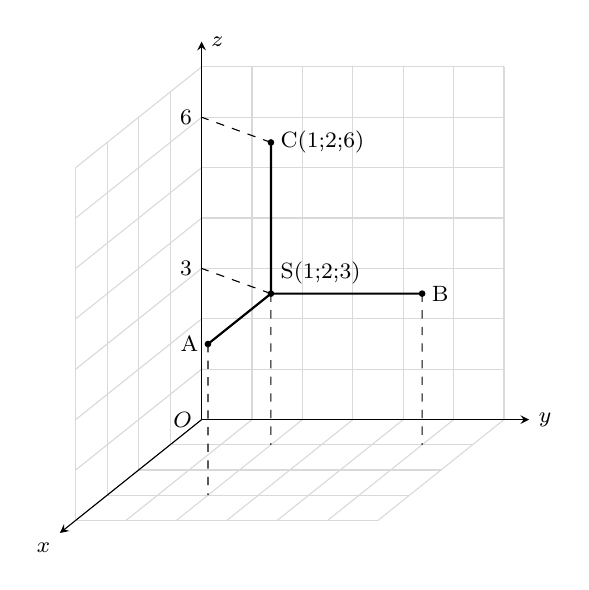
\begin{tikzpicture}[x={(-0.5cm,-0.4cm)}, y={(0.8cm,0cm)}, z={(0cm,0.8cm)}, scale=0.8, font=\footnotesize, >=stealth]
			% --- Cấu hình ---
			\def\xmax{4} \def\ymax{6} \def\zmax{7}
			% --- Vẽ lưới trên 3 mặt phẳng tọa độ ---
			% Mặt phẳng xOz (y=0) - Bức tường bên trái
			\foreach \x in {0,1,...,\xmax} \draw[gray!30] (\x,0,0) -- (\x,0,\zmax);
			\foreach \z in {0,1,...,\zmax} \draw[gray!30] (0,0,\z) -- (\xmax,0,\z);
			
			% Mặt phẳng yOz (x=0) - Bức tường bên phải
			\foreach \y in {0,1,...,\ymax} \draw[gray!30] (0,\y,0) -- (0,\y,\zmax);
			\foreach \z in {0,1,...,\zmax} \draw[gray!30] (0,0,\z) -- (0,\ymax,\z);
			
			% Mặt phẳng xOy (z=0) - Sàn nhà
			\foreach \x in {0,1,...,\xmax} \draw[gray!30] (\x,0,0) -- (\x,\ymax,0);
			\foreach \y in {0,1,...,\ymax} \draw[gray!30] (0,\y,0) -- (\xmax,\y,0);
			% --- Vẽ hệ trục tọa độ ---
			\draw[->] (0,0,0) -- (\xmax+0.5,0,0) node[below left] {$x$};
			\draw[->] (0,0,0) -- (0,\ymax+0.5,0) node[right] {$y$};
			\draw[->] (0,0,0) -- (0,0,\zmax+0.5) node[right] {$z$};
			\node[left] at (0,0,0) {$O$};
			% --- Các điểm ---
			\coordinate (S) at (1,2,3);
			\coordinate (A) at (3,2,3);
			\coordinate (B) at (1,5,3);
			\coordinate (C) at (1,2,6);
			\draw[dashed] (C) -- (0,0,6) node[left] {$6$};
			\draw[dashed] (S) -- (1,2,0); % Chiếu xuống sàn
			\draw[dashed] (3,2,3) -- (3,2,0) (S) -- (0,0,3) node[left] {$3$} (B)--(1,5,0); 
			\draw[thick](C)--(S) (B)--(S) -- (A);
			% --- Tô điểm và nhãn ---
			\foreach \p/\pos/\name in {S/above right/S(1;2;3), A/left/A, B/right/B, C/right/C(1;2;6)}
			\fill (\p) circle (1.5pt) node[\pos] {\name};
	\end{tikzpicture}}
	\loigiai{
		\begin{itemchoice}
			\itemch 
			Dễ thấy $A(3;2;3)$ và $B(1;5;3)$.
			\itemch 
			Ta có $\overrightarrow{SC}=(0;0;3)$ và $\overrightarrow{BC}=(0;-3;3)$. Suy ra $\overrightarrow{SC} \cdot \overrightarrow{BC} = 0 + 0 + 9 = 9$.
			\itemch 
			Ta có $AB =\sqrt{13}$; $AC =\sqrt{13}$;
			$BC =3\sqrt{2}$. \\
			Suy ra $\cos \widehat{BAC} = \dfrac{AB^2 + AC^2 - BC^2}{2\cdot AB \cdot AC} = \dfrac{13 + 13 - 18}{2 \cdot \sqrt{13} \cdot \sqrt{13}} = \dfrac{4}{13}$.
			\itemch 
			Dễ thấy $SB=SC=3$; $SA=2$ và $SA$, $SB$, $SC$ đôi một vuông góc. \\
			Kéo dài $SA$ đến $A'$ sao cho $SA'=3$.\\
			Khi đó hình nón $(N)$ chính là hình nón ngoại tiếp hình chóp tam giác đều $S.A'BC$ có cạnh đáy $BC=3\sqrt{2}$ và khi đó bán kính đáy của nón $(N)$ chính là bán kính đường tròn ngoại tiếp tam giác đều $A'BC$.\\ 
			Suy ra $R = \dfrac{2}{3} \cdot \dfrac{BC\sqrt{3}}{2} = \dfrac{2}{3} \cdot \dfrac{3\sqrt{2} \cdot \sqrt{3}}{2} = \sqrt{6}$.
		\end{itemchoice}
	}
\end{ex}
\Closesolutionfile{ans}

\caukq
\Opensolutionfile{ans}[ans/ans\currfilebase-Phan-III]
\begin{ex}%[2H2V2-6]
	\immini[thm]{Một chú chim bối ca đang ở vị trí $M$ được mô hình hóa trong không gian $Oxyz$ như hình vẽ sau. 
		Gọi $H$ là hình chiếu của $M$ xuống mặt phẳng $(Oxy)$. Biết $OM=50\sqrt{2}$, $\left(\overrightarrow{i}, \overrightarrow{OH}\right)=60^\circ$ và $\left(\overrightarrow{OH}, \overrightarrow{OM}\right)=45^\circ$. Nếu điểm $M(a;b;c)$ thì giá trị của $a+b\sqrt{3}+c$ bằng bao nhiêu?}{	\begin{tikzpicture}[scale=0.85, font=\footnotesize, line join=round, line cap=round, >=stealth]

			\tikzset{chim/.pic={
					\begin{scope}[line width=.05]
						% Đuôi
						\draw [fill=gray]
						(-5.58,-3.02)
						.. controls +(-1.03,-1.24) and +(0.53,-0.37) .. ++(-2.04,-1.46)
						.. controls +(-0.32,-0.13) and +(0.11,-0.32) .. ++(-1.06,0.00)
						.. controls +(-0.53,-0.66) and +(-4.76,-6.01) .. ++(3.78,5.37);
						
						% Đầu  
						\draw[ball color=black!50]
						(-2.28,5.66)
						.. controls +(0.85,2.80) and +(-2.80,2.57) .. ++(7.01,2.14)
						.. controls +(0.37,-0.26) and +(-0.58,0.42) .. ++(3.89,-1.14)
						.. controls +(-0.58,-0.08) and +(1.11,-0.05) .. ++(-2.20,-0.24)
						.. controls +(-0.69,0.03) and +(0.29,0.08) .. ++(-1.67,-0.05);
						% Cánh
						\draw[fill=cyan!40!black!50]
						(0.48,10.05)
						.. controls +(-0.05,1.72) and +(0.42,-0.79) .. ++(-0.79,4.02)
						.. controls +(-0.11,-0.16) and +(0.03,0.37) .. ++(-0.29,-0.66)
						.. controls +(-0.16,1.22) and +(-0.08,1.67) .. ++(-0.74,0.19)
						.. controls +(-0.21,0.66) and +(0.08,1.77) .. ++(-0.69,-0.50)
						.. controls +(-0.40,0.58) and +(0.05,1.48) .. ++(-0.79,-0.40)
						.. controls +(-0.08,0.56) and +(0.13,0.77) .. ++(-0.40,-0.56)
						.. controls +(-0.16,0.24) and +(-0.19,0.90) .. ++(-0.32,-1.03)
						.. controls +(-0.19,0.24) and +(-0.11,0.61) .. ++(-0.32,-0.98)
						.. controls +(-0.21,0.11) and +(-0.11,0.61) .. ++(-0.34,-1.01)
						.. controls +(-0.71,-0.87) and +(-2.94,0.08) .. ++(1.93,-3.47);
						
						\draw[fill=cyan!60!black!70]
						(0.48,10.05)
						.. controls +(0.03,0.42) and +(0.40,-0.11) .. ++(-0.48,1.11)
						.. controls +(-0.21,-0.03) and +(0.08,0.16) .. ++(-0.58,-0.13)
						.. controls +(-0.16,0.11) and +(-0.21,0.50) .. ++(-0.45,-0.21)
						.. controls +(-0.24,-0.03) and +(-0.29,0.45) .. ++(-0.26,-0.61)
						.. controls +(-0.21,-0.08) and +(-0.19,0.21) .. ++(-0.24,-0.56)
						.. controls +(-0.19,-0.05) and +(-0.16,0.24) .. ++(-0.24,-0.42)
						.. controls +(-0.13,-0.13) and +(-0.24,0.19) .. ++(-0.08,-0.48)
						.. controls +(-0.21,-0.05) and +(-0.19,0.05) .. ++(-0.19,-0.32)
						.. controls +(-0.11,-0.16) and +(-0.24,0.34) .. ++(-0.21,-0.53)
						.. controls +(-0.16,-0.08) and +(-0.24,0.13) .. ++(-0.08,-0.34)
						.. controls +(-0.24,-0.19) and +(-0.24,0.21) .. ++(-0.16,-0.61)
						.. controls +(-0.11,-0.19) and +(-0.19,0.00) .. ++(0.11,-0.45)
						.. controls +(-0.16,-0.16) and +(-0.21,0.05) .. ++(0.00,-0.37)
						.. controls +(-0.11,-0.13) and +(-0.16,0.13) .. ++(0.11,-0.48);
						
						\draw [fill=cyan!80!black!90] (.61,8.6)
						.. controls +(.16,.58) and  +(.32,-.05) .. ++(-.14,1.46)
						.. controls +(-.56,-.05) and +(0,1.59) .. ++(-1.83,-2.94);
						%%
						\draw[fill=brown]
						(0.00,0.00)
						.. controls +(1.46,1.43) and +(-0.05,-1.69) .. ++(2.59,4.60)
						.. controls +(-1.90,-0.03) and +(1.40,0.71) .. ++(-2.80,0.40)
						.. controls +(-1.30,-0.93) and +(0.19,1.16) .. ++(-5.13,-6.56)
						.. controls +(-0.69,-0.45) and +(0.24,0.79) .. ++(-1.85,-2.01)
						.. controls +(1.06,-0.16) and +(-1.19,-0.42) .. ++(2.99,1.19)
						.. controls +(0.87,0.16) and +(-0.90,-0.77) .. ++(4.21,2.38);
						\draw[fill=gray!5]
						(2.59,4.60)
						.. controls +(0.19,0.45) and +(-1.40,-0.53) .. ++(2.17,1.77)
						.. controls +(0.29,0.08) and +(-0.69,0.03) .. ++(1.67,0.05)
						.. controls +(-1.03,0.13) and +(0.50,0.08) .. ++(-2.94,0.08)
						.. controls +(-0.40,-0.19) and +(0.37,0.11) .. ++(-1.22,-0.53)
						.. controls +(-0.56,-0.58) and +(0.42,0.40) .. ++(-2.49,-0.98)
						.. controls +(1.40,0.71) and +(-1.90,-0.03) .. ++(2.80,-0.40);
						\draw[fill=cyan]
						(-2.28,5.66)
						.. controls +(0.85,2.80) and +(-2.80,2.57) .. ++(7.01,2.14)
						.. controls +(-0.19,-0.03) and +(0.13,-0.16) .. ++(-0.63,0.00)
						.. controls +(-0.32,-0.29) and +(0.29,0.11) .. ++(-0.93,-0.08)
						.. controls +(-1.08,-0.40) and +(0.98,0.19) .. ++(-2.75,-1.03)
						.. controls +(-0.21,-0.21) and +(0.45,0.13) .. ++(-1.08,-0.34)
						.. controls +(-0.29,0.05) and +(0.87,0.16) .. ++(-1.61,-0.69);
						
						\draw[fill=cyan]
						(3.49,6.51)
						.. controls +(-0.40,-0.19) and +(0.37,0.11) .. ++(-1.22,-0.53)
						.. controls +(-0.56,-0.58) and +(1.40,0.71) .. ++(-2.49,-0.98)
						.. controls +(-1.30,-0.93) and +(0.19,1.16) .. ++(-5.13,-6.56)
						.. controls +(-0.56,-0.21) and +(0.58,0.50) .. ++(-1.93,-1.24)
						.. controls +(0.61,1.93) and +(-2.99,-4.21) .. ++(5.00,8.47)
						.. controls +(0.93,0.05) and +(-0.21,-0.71) .. ++(3.10,0.63)
						.. controls +(1.16,0.69) and +(0.85,0.45) .. ++(2.67,0.21);
						\draw [fill=gray!20]
						(-2.28,5.66)
						.. controls +(0.93,0.05) and +(-0.21,-0.71) .. ++(3.10,0.63)
						.. controls +(0.13,0.26) and +(0.45,0.16) .. ++(-0.40,0.40)
						.. controls +(-0.21,-0.21) and +(0.45,0.13) .. ++(-1.08,-0.34)
						.. controls +(-0.29,0.05) and +(0.87,0.16) .. ++(-1.61,-0.69);
						% Chân 
						\draw[fill=red!60!black!90]
						(-1.68,-1.16)
						.. controls +(1.17,-0.80) and +(0.05,0.95) .. ++(1.20,-1.94)
						.. controls +(-0.16,-0.32) and +(0.53,0.37) .. ++(-0.66,-0.98)
						.. controls +(0.26,0.42) and +(-0.03,-0.29) .. ++(0.42,1.03)
						.. controls +(-0.16,-0.08) and +(0.15,0.13) .. ++(-0.41,-0.42)
						.. controls +(-0.28,0.90) and +(0.21,-0.53) .. ++(-0.41,1.17)
						.. controls +(0.69,0.24) and +(1.22,-0.77) .. ++(-0.59,0.88);
						\draw[fill=red!60!black!90]
						(-2.83,-1.16)
						.. controls +(-0.61,-0.61) and +(-0.71,0.05) .. ++(1.16,-0.87)
						.. controls +(0.34,0.03) and +(0.61,1.56) .. ++(0.29,-2.38)
						.. controls +(0.00,0.58) and +(0.42,-0.42) .. ++(-0.24,1.75)
						.. controls +(0.00,-0.56) and +(0.21,0.21) .. ++(0.03,-1.38)
						.. controls +(0.13,0.53) and +(-0.05,-0.40) .. ++(-0.21,1.32)
						.. controls +(0.29,0.61) and +(-0.58,-0.74) .. ++(-1.61,1.35);
						% Cánh 
						\draw[fill=cyan!80!black!90]
						(-4.54,8.50)
						.. controls +(-2.50,2.16) and +(0.45,-1.24) .. ++(-4.14,5.81)
						.. controls +(-0.11,0.42) and +(-1.69,2.70) .. ++(0.85,-2.70)
						.. controls +(-0.77,0.74) and +(0.50,-0.98) .. ++(-2.09,2.94)
						.. controls +(-0.13,0.42) and +(-1.56,2.12) .. ++(0.95,-2.59)
						.. controls +(-0.90,0.82) and +(0.45,-0.56) .. ++(-1.88,1.93)
						.. controls +(-0.19,0.21) and +(-1.24,1.77) .. ++(0.87,-2.04)
						.. controls +(-0.42,0.29) and +(0.26,-0.32) .. ++(-1.14,1.06)
						.. controls +(-0.19,-0.24) and +(-0.71,1.03) .. ++(0.61,-1.69)
						.. controls +( -0.32,0.21) and +(0.13,-0.13) .. ++(0.79,-1.56)
						.. controls +(-0.21,-0.24) and +(-0.74,0.63) .. ++(-0.90,0.40)
						.. controls +(-0.37,0.16) and +(0.19,0.00) .. ++(0.61,-1.16)
						.. controls +(-0.05,-0.24) and +(-0.58,0.50) .. ++(-0.08,-0.79)
						.. controls +(-0.50,0.32) and +(-0.90,0.98) .. ++(0.29,-0.85)
						.. controls +(-0.32,0.03) and +(-0.95,0.32) .. ++(0.40,-0.79)
						.. controls +(-0.42,-0.03) and +(-1.03,0.19) .. ++(0.26,-0.82)
						.. controls +(-0.42,-0.21) and +(-0.69,0.21) .. ++(0.24,-0.61)
						.. controls +(-0.50,-0.19) and +(-0.71,0.08) .. ++(0.37,-0.74)
						.. controls +(-0.45,-0.29) and +(-0.79,-0.32) .. ++(0.37,-0.56)
						.. controls +(-0.45,-0.34) and +(-0.63,-0.19) .. ++(0.26,-0.69)
						.. controls +(-0.32,-0.29) and +(-0.66,-0.13) .. ++(0.40,-0.58)
						.. controls +(-0.29,-0.24) and +(-0.34,-0.26) .. ++(0.34,-0.50)
						.. controls +(-0.19,-0.29) and +(-0.42,-0.19) .. ++(0.45,-0.42)
						.. controls +(-0.19,-0.26) and +(-0.29,-0.05) .. ++(0.40,-0.48)
						.. controls +(-0.13,-0.24) and +(-0.26,-0.19) .. ++(0.42,-0.29)
						.. controls +(-0.08,-0.32) and +(0.00,0.00) .. ++(0.34,-0.29)
						.. controls +(0.24,-0.05) and +(0.11,-0.16) .. ++(0.45,-0.24)
						.. controls +(0.05,-0.21) and +(-0.11,0.48) .. ++(1.83,1.98)
						.. controls +(1.01,-0.21) and +(-0.37,-0.56) .. ++(0.56,0.34)
						;
						
						\draw [fill=brown!80]
						(-1.04,4.27)
						.. controls +(-1.63,1.69) and +(0.79,-0.59) .. ++(-3.51,4.23)
						.. controls +(-0.75,0.73) and +(0.79,-0.11) .. ++(-2.50,1.85)
						.. controls +(-0.24,0.03) and +(0.05,0.19) .. ++(-0.45,-0.19)
						.. controls +(-0.16,-0.11) and +(-0.19,0.21) .. ++(-0.16,-0.53)
						.. controls +(-0.16,-0.16) and +(-0.19,0.40) .. ++(-0.08,-0.90)
						.. controls +(-0.08,-0.24) and +(-0.29,0.03) .. ++(0.32,-0.53)
						.. controls +(-0.26,-0.24) and +(-0.34,0.08) .. ++(0.16,-0.50)
						.. controls +(0.00,-0.16) and +(-0.34,0.03) .. ++(0.48,-0.34)
						.. controls +(-0.19,-0.13) and +(-0.29,0.08) .. ++(0.21,-0.40)
						
						.. controls +(-0.03,-0.16) and +(-0.32,0.11) .. ++(0.29,-0.45)
						.. controls +(-0.05,-0.13) and +(-0.24,0.00) .. ++(0.34,-0.34)
						.. controls +(-0.16,-0.21) and +(-0.26,0.05) .. ++(0.00,-0.45)
						.. controls +(-0.19,-0.16) and +(-0.32,0.05) .. ++(0.03,-0.42)
						.. controls +(-0.19,-0.19) and +(-0.29,-0.08) .. ++(0.08,-0.40)
						.. controls +(-0.13,-0.29) and +(-0.45,-0.16) .. ++(0.34,-0.29)
						.. controls +(-0.21,-0.32) and +(-0.61,-0.37) .. ++(0.26,-0.50)
						.. controls +(-0.29,-0.37) and +(-1.01,-0.66) .. ++(0.37,-0.21)
						.. controls +(-0.24,-0.32) and +(-1.14,-0.95) .. ++(0.26,-0.26)
						.. controls +(-0.48,-0.77) and +(-0.69,-1.08) .. ++(0.19,-0.26)
						.. controls +(-0.40,-0.79) and +(-0.87,-0.77) .. ++(0.45,-0.34)
						.. controls +(-.59,-.63) and +(-1.11,-1.16) .. ++(.56,.05)
						.. controls +(-.16,-.79) and +(-2.44,-3.82) .. cycle
						;
						\draw [ball color=black] (3.17,7.73)  .. controls +(-.08,.34) and +(.24,.42) .. ++(-.93,-.08)
						.. controls +(-.08,-.82) and +(.21,-.77) .. cycle;
					\end{scope} 
				}
			}
			
			% --- CÁC ĐIỂM VÀ TRỤC TỌA ĐỘ ---
			\coordinate (O) at (0,0);
			\coordinate (A) at (-1.5,-1.2); % Điểm trên Ox
			\coordinate (B) at (3.5,0);      % Điểm trên Oy
			\coordinate (C) at (0,3.5);      % Điểm trên Oz
			\coordinate (H) at ($(A)+(B)$);  % Hình chiếu H
			\coordinate (M) at ($(H)+(0,3.5)$); % Điểm M
			
			% Vẽ trục tọa độ
			\draw[->] (O) -- (-2.2,-1.76) node[below right] {$x$};
			\draw[->] (O) -- (4.8,0) node[below] {$y$};
			\draw[->] (O) -- (0,4.5) node[right] {$z$};
			
			% Vẽ vector đơn vị
			\draw[->] (O) -- (-0.75,-0.6) node[above left=-2pt] {$\overrightarrow{i}$};
			\draw[->] (O) -- (1,0) node[below] {$\overrightarrow{j}$};
			\draw[->] (O) -- (0,1) node[right] {$\overrightarrow{k}$};
			
			% Vẽ các đường gióng (nét đứt)
			\draw[dashed] (A)--(H)--(B);
			\draw[dashed] (H)--(M)--(C);
			\draw[dashed] (O)--(H);
			%\draw[dashed] (A)--(O)--(B); % Nét khuất của trục
			\draw[dashed] (A)--(H);
			
			% Vẽ đường OM
			\draw[thick] (O)--(M);
			
			% Các điểm
			\fill (O) circle (1pt) node[above left] {$O$};
			\fill (M) circle (1.5pt) node[right] {$M$};
			\fill (H) circle (1.5pt) node[below] {$H$};
			\fill (A) circle (1pt) node[left] {$A$};
			\fill (B) circle (1pt) node[below right] {$B$};
			\fill (C) circle (1pt) node[left] {$C$};
			
			% --- CHÈN HÌNH CON CHIM TẠI M ---
			\path (M) pic[scale=0.04, xscale=1, yshift=5mm] {chim};
			
	\end{tikzpicture}}
	\par\shortans[0]{$150$}
	\loigiai{Tam giác $OMH$ vuông cân tại $H$ nên
		$MH = OH = \dfrac{OM}{\sqrt{2}} = \dfrac{50\sqrt{2}}{\sqrt{2}} = 50$.\\
		Tam giác $OAH$ vuông tại $A$ nên
		$OA = OH \cdot \cos 60^\circ = 50 \cdot \dfrac{1}{2} = 25$.\\
		Tam giác $OBH$ vuông tại $B$  nên
		$OB = OH \cdot \sin 60^\circ = 50 \cdot \dfrac{\sqrt{3}}{2} = 25\sqrt{3}$.\\
		Do đó $M\left(25; 25\sqrt{3}; 50\right) \Rightarrow \heva{&a = 25 \\&b = 25\sqrt{3} \\&c = 50.}$ \\
		Vậy $a+b\sqrt{3}+c = 25 + 25\sqrt{3} \cdot \sqrt{3} + 50 = 150$.
	}
\end{ex}

\begin{ex}%[1D1C5-5]
 Biết tổng các nghiệm của phương trình $\sin (\pi \sin 2x)=1$ trên đoạn $[0; 2\pi]$ bằng $a\pi$. Tìm $a$.
\par	\shortans[0]{3}
	\loigiai{
		\begin{eqnarray*}
			&&\sin (\pi \sin 2x)=1\\
			&\Leftrightarrow &\pi \sin 2x = \dfrac{\pi}{2} + k2\pi, \, (k \in \mathbb{Z})\\
			&\Leftrightarrow &\sin 2x = \dfrac{1}{2} + 2k, \, (k \in \mathbb{Z})
	\end{eqnarray*}
		Do $\sin 2x \in [-1; 1]$ nên $-1 \leq \dfrac{1}{2} + 2k \leq 1 \Leftrightarrow -\dfrac{3}{4} \leq k \leq \dfrac{1}{4}$.\\
		$k \in \mathbb{Z}$ nên $k=0$.\\
		Với $k=0$ ta có phương trình $\sin 2x = \dfrac{1}{2} \Leftrightarrow \hoac{&2x = \dfrac{\pi}{6} + l2\pi \\ &2x = \dfrac{5\pi}{6} + l2\pi} \, (l \in \mathbb{Z}) \Leftrightarrow \hoac{&x = \dfrac{\pi}{12} + l\pi \\ &x = \dfrac{5\pi}{12} + l\pi.}$\\
		Do $x \in [0; 2\pi]$ nên $x \in \left\{ \dfrac{\pi}{12}; \dfrac{13\pi}{12}; \dfrac{5\pi}{12}; \dfrac{17\pi}{12} \right\}$.\\\
		Suy ra tổng các nghiệm của phương trình $\sin (\pi \sin 2x)=1$ trên đoạn $[0; 2\pi]$ bằng
		$$\dfrac{\pi}{12} + \dfrac{13\pi}{12} + \dfrac{5\pi}{12} + \dfrac{17\pi}{12} = 3\pi.$$
		Vậy $a=3$.
	}
\end{ex}

\begin{ex}%[2D1C3-6]
	\immini[thm]
	{Mỗi trang của một quyển sách giáo khoa Toán được thiết kế thỏa mãn các tiêu chí sau (trang sách có dạng hình chữ nhật $ABCD$, phần diện tích dùng để trình bày là $MNPQ$).
		\begin{itemize}
			\item Diện tích của trang sách $ABCD$ bằng $491{,}04$ cm$^2$.
			\item Lề trên và lề dưới bằng nhau và bằng $22$ mm.
			\item Lề trái phải lần lượt là $15$ mm và $16$ mm.
		\end{itemize}
		Phần diện tích dùng để trình bày (sau căn chỉnh lề) đạt giá trị lớn nhất, khi đó chu vi mỗi trang sách bằng bao nhiêu? (đơn vị: mm).}
	{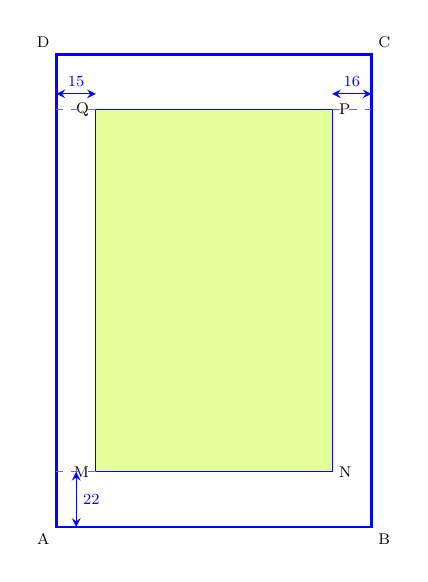
\begin{tikzpicture}[scale=1, font=\footnotesize, >=stealth]
			% Định nghĩa tọa độ các đỉnh hình chữ nhật ngoài
			\coordinate (A) at (0,0);
			\coordinate (B) at (4,0);
			\coordinate (C) at (4,6);
			\coordinate (D) at (0,6);
			
			% Định nghĩa tọa độ các đỉnh hình chữ nhật trong (MNPQ)
			\coordinate (M) at (0.5, 0.7); 
			\coordinate (N) at (3.5, 0.7);
			\coordinate (P) at (3.5, 5.3);
			\coordinate (Q) at (0.5, 5.3);
			
			% Vẽ hình chữ nhật ngoài ABCD
			\draw[thick, blue] (A)--(B)--(C)--(D)--cycle;
			
			% Tô màu và vẽ hình chữ nhật trong MNPQ
			\fill[lime!40] (M)--(N)--(P)--(Q)--cycle;
			\draw[blue] (M)--(N)--(P)--(Q)--cycle;
			\newcommand{\tinynode}[1]{\scalebox{0.7}{#1}}
			\node[below left=-1pt] at (A) {\tinynode{A}};
			\node[below right=-1pt] at (B) {\tinynode{B}};
			\node[above right=-1pt] at (C) {\tinynode{C}};
			\node[above left=-1pt] at (D) {\tinynode{D}};
			
			\node[left=-1pt] at (M) {\tinynode{M}};
			\node[right=-1pt] at (N) {\tinynode{N}};
			\node[right=-1pt] at (P) {\tinynode{P}};
			\node[left=-1pt] at (Q) {\tinynode{Q}};
			
			% Vẽ các đường gióng nét đứt
			\draw[dashed, blue!60, thin] (Q) -- (0, 5.3);
			\draw[dashed, blue!60, thin] (P) -- (4, 5.3);
			\draw[dashed, blue!60, thin] (M) -- (0, 0.7);
			
			% Kích thước 15
			\draw[<->, blue, thin] (0, 5.5) -- (0.5, 5.5) node[midway, above=-1pt] {\tinynode{15}};
			% Kích thước 16
			\draw[<->, blue, thin] (3.5, 5.5) -- (4, 5.5) node[midway, above=-1pt] {\tinynode{16}};
			% Kích thước 22
			\draw[<->, blue, thin] (0.25, 0) -- (0.25, 0.7) node[midway, right=-1pt] {\tinynode{22}};
	\end{tikzpicture}}
	\par\shortans[0]{900}
	\loigiai{
		Đổi $491{,}04$ cm$^2 = 49\,104$ mm$^2$.\\
		Đặt $x$ là chiều dài trang sách ($x>0$, mm).\\
		Chiều rộng trang sách là $\dfrac{49\,104}{x}$ (mm).\\
		Phần trình bày sẽ là phần bên trong trang sách trừ đi các rìa xung quanh.\\
		Chiều dài mới của phần bên trong là $x - 22 - 22 = x - 44$ (mm).\\
		Chiều rộng mới của phần bên trong trang sách là $\dfrac{49\,104}{x} - 15 - 16 = \dfrac{49\,104}{x} - 31$ (mm).\\
		Phần diện tích trình bày cần tìm là
	\begin{eqnarray*}
			S(x) &= &\left(\dfrac{49\,104}{x} - 31\right)(x - 44)\\
			&=&\dfrac{(49\,104 - 31x)(x - 44)}{x}\\
			&=& \dfrac{-31x^2 + 50\,468x - 2\,160\,576}{x}\\
			&= &-31x - \dfrac{2\,160\,576}{x} + 50\,468 \overset{\text{AM-GM}}{\leq} -2\sqrt{31x \cdot \dfrac{2\,160\,576}{x}} + 50\,468 = 34\,100.
		\end{eqnarray*}
		Dấu \lq\lq$=$\rq\rq\, xảy ra khi $$31x = \dfrac{2\,160\,576}{x} \Leftrightarrow x^2 = 69\,696 \Leftrightarrow x = 264.$$
		Vậy chu vi mỗi trang sách là $2\left(\dfrac{49\,104}{x} + x\right) = 2\left(\dfrac{49\,104}{264} + 264\right) = 900$ (mm).
	}
\end{ex}

\begin{ex}%[1H8V7-6]
	\immini[thm]{ Một vật lưu niệm làm bằng thủy tinh có dạng hình lăng trụ đều có đáy $ABCD$ là hình vuông cạnh $AB=10$ (cm). Phía bên trong làm bằng nhựa đặc là hình chóp cụt đều $MNPQ.ABCD$ có $MN=5$ (cm) và chiều cao bằng chiều cao của lăng trụ như hình vẽ. Biết rằng khoảng cách từ điểm $B$ đến mặt phẳng $(CDQP)$ bằng $3\sqrt{10}$ (cm). Phần khoảng trống bên trong vật lưu niệm người ta bơm chất lỏng có màu sắc (xem độ dày thành vật thể không đáng kể). 	Khi đó thể tích phần chất lỏng bơm vào là $\dfrac{a}{b}$ (lít) với $\dfrac{a}{b}$ là phân số tối giản. Tìm $a+b$.}{	\begin{tikzpicture}[line join=round, line cap=round, scale=0.6, font=\footnotesize]
			% Định nghĩa các tọa độ
			\coordinate (A) at (-0.2,0);
			\coordinate (B) at (-2.5,-2);
			\coordinate (D) at (5,0);
			\coordinate (C) at ($(B)+(D)-(A)$);
			\def\h{5} % Chiều cao
			\coordinate (AA) at ($(A)+(0,\h)$);
			\coordinate (BB) at ($(B)+(0,\h)$);
			\coordinate (CC) at ($(C)+(0,\h)$);
			\coordinate (DD) at ($(D)+(0,\h)$);
			
			% Định nghĩa các điểm của hình chóp cụt phía trên (tỉ lệ 5/10 = 1/2)
			\coordinate (O) at ($(AA)!0.5!(CC)$); % Tâm nắp trên
			\coordinate (M) at ($(O)!0.5!(AA)$);
			\coordinate (N) at ($(O)!0.5!(BB)$);
			\coordinate (P) at ($(O)!0.5!(CC)$);
			\coordinate (Q) at ($(O)!0.5!(DD)$);
			
			% Tô màu
			% Mặt bên chóp cụt (trái và phải)
			\fill[cyan!10] (B)--(C)--(P)--(N)--cycle;
			\fill[cyan!20] (C)--(D)--(Q)--(P)--cycle;
			% Nắp trên (trong)
			\fill[purple!20] (M)--(N)--(P)--(Q)--cycle;
			
			% Vẽ các cạnh khuất (nét đứt)
			\draw[dashed](N)--(B)--(A)--(D)--(Q) (P)--(C) (AA)--(A)--(M);
			\draw (AA)--(CC)--(BB)--(DD)--(AA)--(BB)--(B)--(C)--(CC)--(DD)--(D)--(C)  (M)--(N)--(P)--(Q)--(M);
			% Vẽ các điểm và gán nhãn
			\foreach \x/\g/\t in { A/left/A,B/left/B,C/right/C,D/right/D,AA/above/A',BB/left/B', CC/right/C',DD/right/D',M/left/M,
				N/above left/N,P/right/P,Q/above/Q}
			{\draw[fill=white] (\x) circle (1.5pt) node[\g] {$\t$};}
	\end{tikzpicture}}
\par\shortans[0]{21}
	\loigiai{
		\begin{center}
			\begin{tikzpicture}[line join=round, line cap=round, scale=0.6, font=\footnotesize]
				% --- 1. ĐỊNH NGHĨA TỌA ĐỘ ---
				\coordinate (A) at (-0.2,0);
				\coordinate (B) at (-2.5,-2);
				\coordinate (D) at (5,0);
				\coordinate (C) at ($(B)+(D)-(A)$);
				\def\h{5} % Chiều cao
				
				\coordinate (AA) at ($(A)+(0,\h)$);
				\coordinate (BB) at ($(B)+(0,\h)$);
				\coordinate (CC) at ($(C)+(0,\h)$);
				\coordinate (DD) at ($(D)+(0,\h)$);
				
				% Các điểm của hình chóp cụt (tỉ lệ 1/2)
				\coordinate (O) at ($(AA)!0.5!(CC)$); 
				\coordinate (M) at ($(O)!0.5!(AA)$);
				\coordinate (N) at ($(O)!0.5!(BB)$);
				\coordinate (P) at ($(O)!0.5!(CC)$);
				\coordinate (Q) at ($(O)!0.5!(DD)$);
				
				% --- 2. DỰNG HÌNH PHỤ ---
				% H là giao điểm của PQ kéo dài và B'C'
				\coordinate (H) at (intersection of P--Q and BB--CC);
				
				% Lấy điểm L bất kỳ trên CH (tỉ lệ 0.75 để nhìn rõ và đẹp)
				\coordinate (L) at ($(C)!0.6!(H)$);
				
				% --- 3. TÔ MÀU (FILL) ---
				\fill[cyan!10] (B)--(C)--(P)--(N)--cycle;
				\fill[cyan!20] (C)--(D)--(Q)--(P)--cycle;
				\fill[purple!20] (M)--(N)--(P)--(Q)--cycle;
				
				% --- 4. VẼ NÉT ĐỨT (DASHED) ---
				\draw[dashed] (B)--(A)--(D) (A)--(AA); 
				\draw[dashed] (A)--(M);                 
				\draw[dashed] (P)--(C); % PC nét đứt
				
				% --- 5. VẼ NÉT LIỀN (SOLID) ---
				\draw (B)--(C)--(D);
				\draw (BB)--(CC)--(DD)--(AA)--(BB); 
				\draw (BB)--(B) (CC)--(C) (DD)--(D) (AA)--(CC) (BB)--(DD); 
				\draw (M)--(N)--(P)--(Q)--cycle; % MNPQ nét liền
				\draw (N)--(B);
				\draw (Q)--(D);
				
				% --- 6. VẼ CÁC ĐƯỜNG LỜI GIẢI ---
				\draw (Q)--(H); 
				\draw (C)--(H); 
				\draw (B)--(L); 
				
				% --- 7. KÍ HIỆU VUÔNG GÓC DÙNG PIC ---
				\pic[draw, angle radius=2mm]{right angle=B--L--C};
				
				% --- 8. VẼ ĐIỂM VÀ NHÃN ---
				\foreach \x/\g/\t in {
					A/left/A,
					B/left/B,
					C/right/C,
					D/right/D,
					AA/above/A',
					BB/left/B',
					CC/right/C',
					DD/right/D',
					M/left/M,
					N/above left/N,
					P/right/P,      
					Q/above/Q,
					H/below left/H,      
					L/below right/L       
				}
				{
					\draw[fill=white] (\x) circle (1.5pt) node[\g] {$\t$};
				}
			\end{tikzpicture}
		\end{center}
		Kéo dài $PQ$ cắt $B'C'$ tại $H$, kẻ $BL \perp CH$. \\
		Mà $CD \perp BL \left( CD \perp (BCC'B') \right)$ nên $BL \perp (CDQP)$. \\
		Suy ra $\mathrm{d}[B;(CDQL)] = BL = 3\sqrt{10}$. \\
		Ta có $\triangle LBC \sim \triangle C'CH \Rightarrow \dfrac{BL}{C'C} = \dfrac{BC}{CH} \Rightarrow \dfrac{3\sqrt{10}}{C'C} = \dfrac{10}{\sqrt{CC'^2 + 2{,}5^2}} \Rightarrow CC' = \dfrac{15}{2}.$ \\
		Khi đó $V_{\text{chóp cụt}} = \dfrac{CC'}{3} \left( S_1 + S_2 + \sqrt{S_1 . S_2} \right) = \dfrac{5}{2} \left( 10^2 + 5^2 + \sqrt{10^2 . 5^2} \right) = \dfrac{875}{2}$ cm$^3$.\\
		$V_{\text{chất lỏng}} = 10^2 \cdot \dfrac{15}{2} - V_{\text{chóp cụt}} = \dfrac{625}{2} $ cm$^3$ $= \dfrac{5}{16}$ lít. \\
		Vậy $a=5$, $b=16$ do đó $ a+b=21$.
	}
\end{ex}

\begin{ex}%[2H2C2-6]
	Cho hình lăng trụ $ABC.A'B'C'$. Biết rằng $A'.ABC$ là tứ diện đều có cạnh bằng $2$ (cm). Cùng một thời điểm, hai chất điểm xuất phát từ $C'$ và $A$ di chuyển trên đoạn $C'A'$ và $AM$ (với $M$ là trung điểm của đoạn $BC$) với tốc độ lần lượt là $2$ (m/s) và $2\sqrt{3}$ (m/s). Tìm thời điểm (tính theo giây) mà khoảng cách giữa hai chất điểm là ngắn nhất? \textit{(làm tròn đến hàng phần trăm)}.
	\par\shortans[0]{0{,}57}
	\loigiai{
	\immini{
		Gọi $G$ là trọng tâm tam giác đều $ABC$. Chọn hệ tọa độ $Oxyz$ với gốc tọa độ tại $M$, tia $Ox$ trùng với tia $OC$, tia $Oy$ trùng với tia $OA$, tia $Oz$ cùng hướng với tia $GA'$. \\ 
		Từ đó ta có tọa độ các điểm $M$, $C$, $A$, $A'$ lần lượt là 
		$$M(0;0;0),\, C(1;0;0),\, A\left(0;\sqrt{3};0\right),\, A'\left(0;\dfrac{\sqrt{3}}{3};\dfrac{2\sqrt{6}}{3}\right).$$
		Gọi $P$, $Q$ lần lượt là vị trí của hai chất điểm tại thời điểm $t$ (giây).}{
	\begin{tikzpicture}[scale=0.8,>=stealth, line join=round, line cap=round, font=\footnotesize]
	\coordinate (A) at (-2.5, -0.5);   % Góc trái dưới
	\coordinate (C) at (0, -2);        % Góc dưới cùng
	\coordinate (B) at (2.5, -0.5);    % Góc phải dưới
	\coordinate (M) at ($(B)!0.5!(C)$); 
	\coordinate (G) at ($(A)!2/3!(M)$);
	\coordinate (AA) at ($(G)+(0,4.5)$); 
	\coordinate (v) at ($(AA)-(A)$);	
	% Các đỉnh còn lại
	\coordinate (BB) at ($(B)+(v)$);
	\coordinate (CC) at ($(C)+(v)$);
	\coordinate (MM) at ($(M)+(v)$); 
	\coordinate (Z) at ($(AA)!0.33!(MM)$); 
	
	\coordinate (P) at ($(CC)!0.3!(AA)$); % P trên C'A'
	\coordinate (Q) at ($(A)!0.4!(M)$);   % Q trên AM
	
	\draw[dashed](AA)--(G) (A)--(B) (A)--(M);
	\draw (CC)--(AA)--(BB)--(CC)--(C) (AA)--(A) (B)--(BB);
	\draw (A)--(C)--(B);
	\draw[dashed](M)--(A)--(B);
	
	% Hệ trục tọa độ
	\draw [->](A)--($(M)!1.4!(A)$)node[above]{$y$};
	\draw [->](M)--($(M)!2!(C)$)node[above left]{$x$}; 
	\draw [->,dashed](M)--($(M)!1.1!(Z)$)node[above left]{$z$}; 
	
	% Vẽ vector chuyển động
	\draw[->,line width=1pt, red] (CC)--(P) node[midway, above right]{$\overrightarrow{C'P}$};
	\draw[->,line width=1pt, blue] (A)--(Q) node[midway, below left]{$\overrightarrow{AQ}$};
	
	% Vẽ các điểm
	\foreach \p/\pos/\lab in {
		A/below left/A, B/right/B, C/below/C, M/below/M,
		AA/above/A', BB/right/B', CC/right/C',
		G/below/G
	}
	\draw[fill=white] (\p) circle (1.5pt) node[\pos] {$\lab$};
	% Tô đậm 2 điểm chuyển động
	\fill[red] (P) circle (1.5pt) node[above]{$P$};
	\fill[blue] (Q) circle (1.5pt) node[below]{$Q$};
	
\end{tikzpicture}		
		}\noindent
Ta có $\overrightarrow{C'P}=\dfrac{C'P}{C'A'}\cdot\overrightarrow{C'A'}=\dfrac{2t}{2}\cdot \left(-1;\sqrt{3};0\right)=\left(-t;t\sqrt{3};0\right)$.\\
Suy ra $P\left(1-t;-\dfrac{2\sqrt{3}}{3}+t\sqrt{3};\dfrac{2\sqrt{6}}{3}\right)$.\\
		Lại có $\overrightarrow{AQ}=\dfrac{AQ}{AM}\cdot \overrightarrow{AM} = \dfrac{2\sqrt{3}t}{\sqrt{3}}\cdot \left(0;-\sqrt{3};0\right) = \left(0;-2t\sqrt{3};0\right)$.\\
		Suy ra $Q\left(0;\sqrt{3}-2t\sqrt{3};0\right)$.\\
		Khi đó
		$$
			PQ^2 = (t-1)^2 + \left(\dfrac{5\sqrt{3}}{3}-3t\sqrt{3}\right)^2 + \dfrac{8}{3}
			= 28t^2-32t+12.
		$$
		Khoảng cách $PQ$ ngắn nhất khi $28t^2-32t+12$ nhỏ nhất.\\ Xét đỉnh parabol ta có $t=\dfrac{32}{2\cdot 28} = \dfrac{4}{7} \approx 0{,}57$.
	}
\end{ex}

\begin{ex}%[1D9V1-3]
Cho hai hộp đựng bi, đựng hai loại bi là bi xanh và bi đỏ, tổng số bi của cả hai hộp là $15$ bi và hộp thứ nhất đựng nhiều bi hơn hộp thứ hai, đồng thời số bi xanh ở hộp một nhiều hơn số bi xanh ở hộp hai. Lấy ngẫu nhiên từ mỗi hộp một bi. Nếu xác suất để lấy được $2$ bi xanh là $\dfrac{5}{28}$ thì xác suất để lấy được $2$ bi đỏ là $\dfrac{a}{b}$ với $\dfrac{a}{b}$ là phân số tối giản. Tìm $D=a+b$.
	\par\shortans[0]{71}
	\loigiai{
		Gọi số bi của hộp $1$ và $2$ lần lượt là $m$, $n$ suy ra $ m+n=15$; $m>n$.\\
		Gọi số bi xanh của hộp $1$ và $2$ lần lượt là $x$, $y$, $(x>y)$.\\
		Theo giả thiết $\dfrac{x}{m}\cdot \dfrac{y}{n}=\dfrac{5}{28}=\dfrac{10}{56} \Rightarrow mn=56=7\cdot 8 \Rightarrow \heva{&m=8\\&n=7.}$\\
		Ta có $xy=10=2\cdot 5 \Rightarrow \heva{&x=5\\&y=2.}$\\
		Vậy số bi xanh của hộp $1$ và $2$ lần lượt là $5$; $2$.\\
		Xác suất để lấy được $2$ bi đỏ là $\dfrac{3}{8}\cdot \dfrac{5}{7}=\dfrac{15}{56}\Rightarrow a+b=71$.
	}
\end{ex}

\Closesolutionfile{ans}
\Closesolutionfile{ansbook}
% \begin{indapan}
%     {ans/ans\currfilebase}
% \end{indapan}
